\documentclass{article}
\usepackage[utf8]{inputenc} %кодировка
\usepackage[T2A]{fontenc}
\usepackage[english,russian]{babel} %русификатор 
\usepackage{mathtools} %библиотека матеши
\usepackage[left=1cm,right=1cm,top=2cm,bottom=2cm,bindingoffset=0cm]{geometry} %изменение отступов на листе
\usepackage{amsmath}
\usepackage{graphicx} %библиотека для графики и картинок
\graphicspath{}
\DeclareGraphicsExtensions{.pdf,.png,.jpg}
\usepackage{subcaption}
\usepackage{pgfplots}
\usepackage{float}
\usepackage{listings}


\lstset{
    numbers=left,            % Нумерация строк слева
    numberstyle=\tiny,       % Размер шрифта для номеров строк
    stepnumber=1,            % Нумеровать каждую строку
    numbersep=5pt,           % Расстояние между номерами и кодом
    backgroundcolor=\color{white},  % Цвет фона
    showspaces=false,        % Не показывать пробелы
    showstringspaces=false,  % Не показывать пробелы в строках
    showtabs=false,          % Не показывать табуляцию
    frame=single,            % Рамка вокруг кода
    tabsize=2,               % Размер табуляции
    breaklines=true,         % Автоматический перенос строк
    breakatwhitespace=true   % Переносить строки только по пробелам
}

\begin{document}
% НАЧАЛО ТИТУЛЬНОГО ЛИСТА
\begin{center}
    \Large
    Федеральное государственное автономное \\
    образовательное учреждение высшего образования \\ 
    «Научно-образовательная корпорация ИТМО»\\
    \vspace{0.5cm}
    \large
    Факультет программной инженерии и компьютерной техники \\
    Направление подготовки 09.03.04 Программная инженерия \\
    \vspace{1cm}
    \Large
    \textbf{Отчёт по лабораторной работе №1} \\
        По дисциплине «Системы ввода-вывода» ( семестр 6)\\
    \large
    \vspace{8cm}

    \begin{minipage}{.33\textwidth}
    \end{minipage}
    \hfill
    \begin{minipage}{.4\textwidth}
    
        \textbf{Студент}: \vspace{.1cm} \\
        \ Дениченко Александр P3212\\
        \ Разинкин Александр P3207\\
        \textbf{Практик}:  \\
        \ Табунщик Сергей Михайлович
    \end{minipage}
    \vfill
Санкт-Петербург\\ 2025 г.
\end{center}
\pagestyle{empty}
% КОНЕЦ ТИТУЛЬНОГО ЛИСТА 
\newpage
\pagestyle{plain}

\section*{Задачи}
Лабораторная работа:

1. Реализовать функцию putchar вывода данных в консоль

2. Реализовать функцию getchar для получения данных из консоли

3. На базе реализованных функций putchar и getchar написать программу,
позволяющую вызывать определенным вариантом функции OpenSBI
посредством взаимодействия пользователя через меню

4. Запустить программу и выполнить вызов пунктов меню, получив результаты их
работы

5. Оформить отчет по работе в электронном формате
\\ \\
Вариант - 1:

1. Get SBI specification version

2. Get number of counters

3. Get details of a counter (должно быть возможно задавать
номер счетчика)

4. System Shutdown

\begin{lstlisting}[caption={run.sh}, label={lst:example}]
    set -xue

    QEMU=qemu-system-riscv32

    CC=/opt/homebrew/opt/llvm/bin/clang
    CFLAGS="-std=c11 -O2 -g3 -Wall -Wextra --target=riscv32 -ffreestanding -nostdlib"

    $CC $CFLAGS -Wl,-Tkernel.ld -Wl,-Map=kernel.map -o kernel.elf kernel.c

    $QEMU -machine virt -bios default -nographic -serial mon:stdio --no-reboot -kernel kernel.elf
\end{lstlisting}
    
\begin{lstlisting}[caption={kernel.h}, label={lst:example}]
    #pragma once

    struct sbiret {
        long error;
        long value;
    };
\end{lstlisting}

\begin{lstlisting}[caption={kernel.ld}, label={lst:example}]
    ENTRY(boot)

    SECTIONS {
        . = 0x80200000;

        .text :{
            KEEP(*(.text.boot));
            *(.text .text.*);
        }

        .rodata : ALIGN(4) {
            *(.rodata .rodata.*);
        }

        .data : ALIGN(4) {
            *(.data .data.*);
        }

        .bss : ALIGN(4) {
            __bss = .;
            *(.bss .bss.* .sbss .sbss.*);
            __bss_end = .;
        }

        . = ALIGN(4);
        . += 128 * 1024; /* 128KB */
        __stack_top = .;
    }
\end{lstlisting}

\begin{lstlisting}[caption={kernel.ld}, label={lst:example}]
    #include "kernel.h"

    extern char __bss[], __bss_end[], __stack_top[];

    struct sbiret sbi_call(long arg0, long arg1, long arg2, long arg3, long arg4,
        long arg5, long fid, long eid) {
        register long a0 __asm__("a0") = arg0;
        register long a1 __asm__("a1") = arg1;
        register long a2 __asm__("a2") = arg2;
        register long a3 __asm__("a3") = arg3;
        register long a4 __asm__("a4") = arg4;
        register long a5 __asm__("a5") = arg5;
        register long a6 __asm__("a6") = fid;
        register long a7 __asm__("a7") = eid;

        __asm__ __volatile__("ecall"
            : "=r"(a0), "=r"(a1)
            : "r"(a0), "r"(a1), "r"(a2), "r"(a3), "r"(a4), "r"(a5),
                "r"(a6), "r"(a7)
            : "memory");
        return (struct sbiret){.error = a0, .value = a1};
    }

    long sbi_call_long(long arg0, long arg1, long arg2, long arg3, long arg4,
        long arg5, long fid, long eid) {
        register long a0 __asm__("a0") = arg0;
        register long a1 __asm__("a1") = arg1;
        register long a2 __asm__("a2") = arg2;
        register long a3 __asm__("a3") = arg3;
        register long a4 __asm__("a4") = arg4;
        register long a5 __asm__("a5") = arg5;
        register long a6 __asm__("a6") = fid;
        register long a7 __asm__("a7") = eid;

        __asm__ __volatile__("ecall"
            : "=r"(a0), "=r"(a1)
            : "r"(a0), "r"(a1), "r"(a2), "r"(a3), "r"(a4), "r"(a5),
                "r"(a6), "r"(a7)
            : "memory");
        return a0;
    }

    void putchar(char ch) {
        sbi_call(ch, 0, 0, 0, 0, 0, 0, 1 /* Console Putchar */);
    }

    char getchar(void) {
        for (;;) {
            long ch = sbi_call_long(0, 0, 0, 0, 0, 0, 0, 2);
            if (ch != -1 && ch != 0) {
                return ch;
            }
        }
    }

    long read_number(void) {
        long number = 0; 
        int sign = 1;    
        char ch;

        while ((ch = getchar()) != '\n') { 
            if (ch < '0' || ch > '9') {
                putchar('E'); 
                putchar('\n');
                return 0; 
            }

            number = number * 10 + (ch - '0'); 
        }

        return number * sign; 
    }

    void show_sbi_version(void) {
        struct sbiret result = sbi_call(0, 0, 0, 0, 0, 0, 0, 0x10);

        long number = result.value & 0xFFFFFF;
        char high = (number >> 16) & 0xFF;
        char mid = (number >> 8) & 0xFF;
        char low = number & 0xFF;

        putchar('0' + high + mid + low);

        putchar('.');

        putchar('0' + (result.value >> 24));    
    }

    void show_num_counter(void) {
        const char *s = "\n\nCount: ";
        for (int i = 0; s[i] != '\0'; i++) {
            putchar(s[i]);
        }

        struct sbiret result = sbi_call(0, 0, 0, 0, 0, 0, 0, 0x504D55);

        long number = result.value;

        if (number == 0) {
            putchar('0');
            return;
        }

        char digits[10]; 
        int count = 0;

        while (number > 0) {
            digits[count] = '0' + (number % 10); 
            number /= 10; 
            count++;
        }

        for (int i = count - 1; i >= 0; i--) {
            putchar(digits[i]);
        }

    }

    void print_string(const char *s) {
        for (int i = 0; s[i] != '\0'; i++) {
        putchar(s[i]);
        }
    }
    
    void print_number(long num) {
        char buffer[32];
        int i = 0;
    
        if (num == 0) {
        putchar('0');
        return;
        }
    
        if (num < 0) {
        putchar('-');
        num = -num;
        }
    
        while (num > 0) {
        buffer[i++] = '0' + (num % 10);
        num /= 10;
        }
    
        while (--i >= 0) {
        putchar(buffer[i]);
        }
    }

    void show_counter(void) {

        int counter_num = 0;
        char digit = getchar();
        putchar(digit);
        if (digit >= '0' && digit <= '9') {
        counter_num = digit - '0';
        char next = getchar();
        if (next >= '0' && next <= '9') {
            putchar(next);
            counter_num = counter_num * 10 + (next - '0');
        }
        }
        print_string("\n");

        struct sbiret info = sbi_call(counter_num, 0, 0, 0, 0, 0, 1, 0x504D55);

        unsigned long counter_info = info.value;
        unsigned long csr = counter_info & 0xFFF;           // bits [11:0]
        unsigned long width = (counter_info >> 12) & 0x3F;  // bits [17:12]
        unsigned long type = counter_info >> (sizeof(long) * 8 - 1); // highest bit

        print_string("Counter details:\n");
        print_string("Type: ");
        print_string(type ? "Firmware" : "Hardware");
        print_string("\n");
        
        if (type == 0) {  // Only show CSR and width for hardware counters
        print_string("CSR number: 0x");
        print_number(csr);
        print_string("\nWidth: ");
        print_number(width + 1);  // Width is stored as (actual width - 1)
        print_string(" bits\n");
        }
    }

    void system_shutdown(void) {
        const char *s = "\n\nTurn off!\n";
        for (int i = 0; s[i] != '\0'; i++) {
            putchar(s[i]);
        }

        sbi_call(0, 0, 0, 0, 0, 0, 0, 8);
    }

    void kernel_main(void) {
        for (;;) {
            switch (getchar()) {
                case '1':
                    show_sbi_version();
                    putchar('\n');
                    break;
                case '2':
                    show_num_counter();
                    putchar('\n');
                    break;
                case '3':
                    show_counter();
                    break;
                case '4':
                    system_shutdown();
                    break;
                default:
                    const char *s = "\n\nUnknown symbol";
                    for (int i = 0; s[i] != '\0'; i++) {
                        putchar(s[i]);
                    }
                    putchar('\n');
            }
        }
    }

    __attribute__((section(".text.boot")))
    __attribute__((naked))
    void boot(void) {
        __asm__ __volatile__(
            "mv sp, %[stack_top]\n" 
            "j kernel_main\n"      
            :
            : [stack_top] "r" (__stack_top)
        );
    }
\end{lstlisting}

\section{Тестирование системы}
Ввод -> 1
\begin{center}
    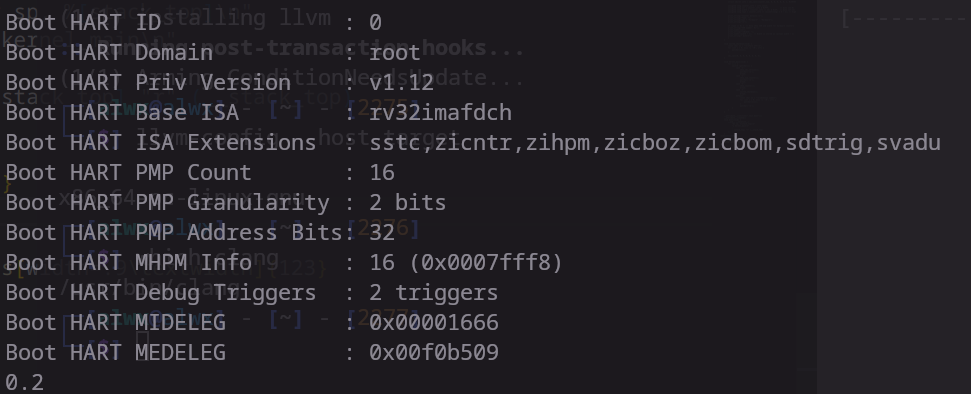
\includegraphics[width=.9\textwidth]{1}
\end{center}

Ввод -> 2
\begin{center}
    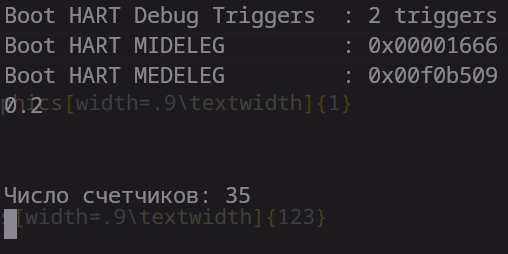
\includegraphics[width=.7\textwidth]{2}
\end{center}


Ввод -> 3 3
\begin{center}
    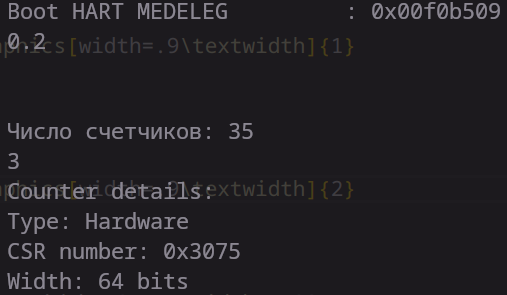
\includegraphics[width=.7\textwidth]{3}
\end{center}

Ввод -> 4 
\begin{center}
    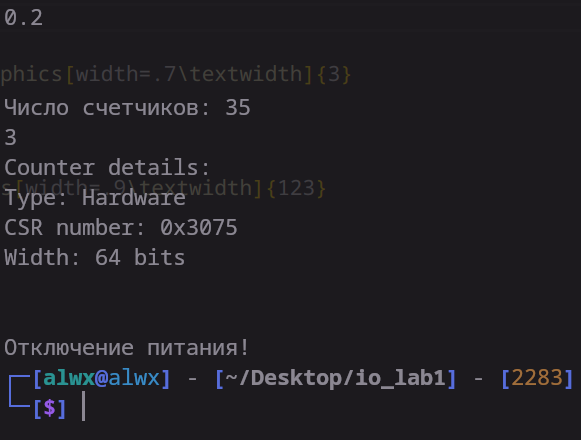
\includegraphics[width=.7\textwidth]{4}
\end{center}
(в отчёте вставлен код со всем выводом на en локали, функционал не менялся)

\end{document}
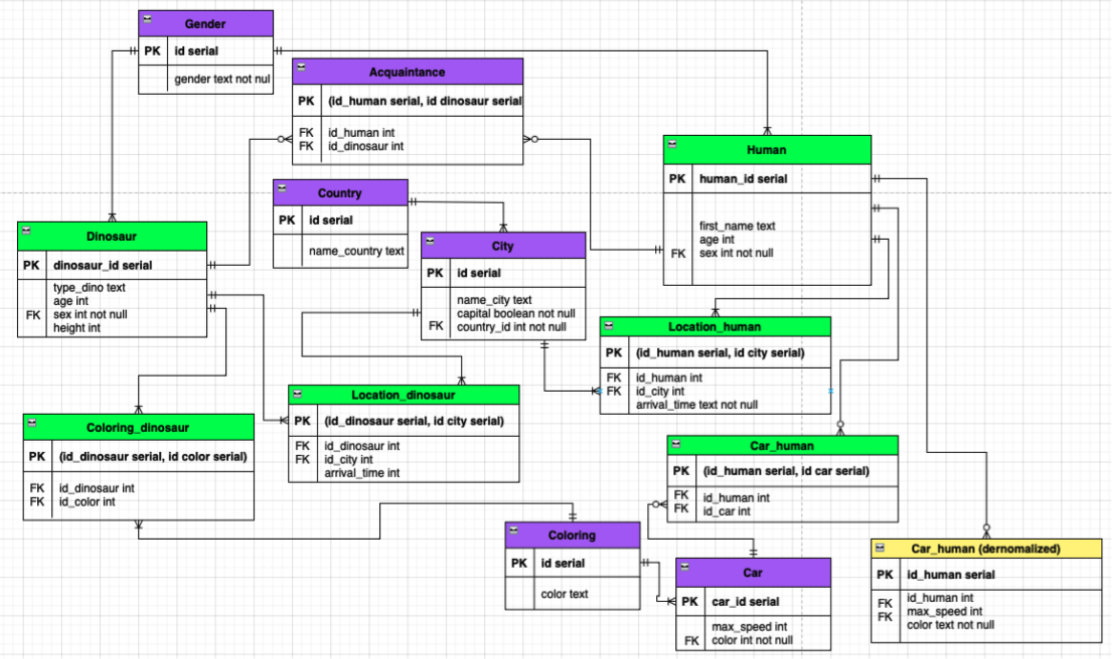
\includegraphics[width=.9\textwidth]{123}